% Standard Article Definition
\documentclass[]{article}

% Page Formatting
\usepackage[margin=1in]{geometry}
\setlength\parindent{0pt}

% Graphics
\usepackage{graphicx}

% Math Packages
\usepackage{physics}
\usepackage{amsmath, amsfonts, amssymb, amsthm}
\usepackage{mathtools}

% Extra Packages
\usepackage{pdfpages}
\usepackage{hyperref}
% \usepackage{listings}

% Section Heading Settings
\usepackage{enumitem}
% \renewcommand{\theenumi}{\alph{enumi}}
\renewcommand*{\thesection}{Problem \arabic{section}}
\renewcommand*{\thesubsection}{\alph{subsection})}
\renewcommand*{\thesubsubsection}{}%\quad \quad \roman{subsubsection})}

\newcommand{\Problem}{\subsubsection*{\textbf{PROBLEM:}}}
\newcommand{\Solution}{\subsubsection*{\textbf{SOLUTION:}}}
\newcommand{\Preliminaries}{\subsubsection*{\textbf{PRELIMINARIES:}}}

%Custom Commands
\newcommand{\N}{\mathbb{N}}
\newcommand{\Z}{\mathbb{Z}}
\newcommand{\Q}{\mathbb{Q}}
\newcommand{\R}{\mathbb{R}}
\newcommand{\C}{\mathbb{C}}

\newcommand{\SigAlg}{\mathcal{S}}

\newcommand{\Rel}{\mathcal{R}}

% \newcommand{\toI}{\xrightarrow{\textsf{\tiny I}}}
% \newcommand{\toS}{\xrightarrow{\textsf{\tiny S}}}
% \newcommand{\toB}{\xrightarrow{\textsf{\tiny B}}}

\newcommand{\divisible}{ \ \vdots \ }
\newcommand{\st}{\ : \ }

% Theorem Definition
\newtheorem{definition}{Definition}
\newtheorem{assumption}{Assumption}
\newtheorem{theorem}{Theorem}
\newtheorem{lemma}{Lemma}
\newtheorem{proposition}{Proposition}
\newtheorem{remark}{Remark}
% \newtheorem{example}{Example}
% \newtheorem{counterExample}{Counter Example}


%opening
\title{MATH 6301 Real Analysis I \\ Homework 5}
\author{Jonas Wagner\\ jonas.wagner@utdallas.edu}
\date{2022, December 1\textsuperscript{st}}

\begin{document}

\maketitle

\tableofcontents

\includepdf[pages={2}]{math6301a5-2022.pdf}

% Problem 1 ----------------------------------------------
\newpage
\section{}
\Problem
Let $(X, \SigAlg,\mu)$ be a measure space, $E \in \SigAlg$, and $f : E \to \overline{\R}$ a summable function.                                                                                          
Show that \[
\mu\{x \in E \st \abs{f(x)} = \infty\} = 0
\]

\Preliminaries
\begin{definition}
    Let $f : [a,b] \to [0,\infty)$ be a measuable function.
    The \emph{\underline{integral}} of $f$ (which can be equal to $\infty$) on a measurable set $E \subset [a,b]$ with respect to measure $\mu$ is defined by \[
        \int_{E} f(x) \dd \mu(x) := \sup\qty{
            \int_{E} s \dd \mu : \forall_{x \in X} 0 \leq s(x) \leq f(x)
        }
    \] 
    
    Notes: 
    \begin{itemize}
        \item Each $s(x)$ can be considered a set of piecewise simple functions that approximate $f(x)$.
        \item If $\int_{E} f \dd \mu < \infty$ then $f$ is said to be \emph{\underline{summable}} on $E$.
        \item We can look at functions defined to $\R$ as opposed to just $[0,\infty)$ as two functions defined when positive and negative ($f_{+}$ and $f_{-}$) and then the integral is just the sum of positive minus the negative.
        \item If $E \subset [a,b]$ is a measurable set, then we can use the charectoristic/indication function of $E$, $\chi_E$ (1 if included in the set, otherwise 0), and do the integral as \[
            \int_{E} f(x) \dd \mu(x) := \int_{a}^{b} \chi_{E}(x) f(x) \dd \mu(x)
        \]
    \end{itemize}    
\end{definition}

\Solution

The solution to this problem revolves around the fact that $f$ is defined as a summable function. 
Although defined unto the entire space $\overline{\R}$, in order for the condition to be true, $\abs{f(x)} = \infty$ must be accompanied by $\chi_E(x) = 0$ ($x \neq E$) or be individual/distinct/(satisfying $\mu\{\cdot\} = 0$).

In a more straight forward manor, we have that $f$ summable on $E$ implies $f_{+}$ and $f_{-}$ summable on $E$ meaning $f_{+}$ and $f_{-}$ are bounded almost anywhere on $E$ which therefore implies $\abs{f} = f_{+} + f_{-}$ is also bounded almost anywhere on $E$.
This then implies that the measure where $\abs{f}(x) = \infty$ is 0.
i.e.
\begin{align*}
    \int_{E} f \dd{\mu} < \infty 
    &\implies 
    \int_{E} f_{+} \dd{\mu},\int_{E} f_{-} \dd{\mu} < \infty
    \implies\\ &\implies
    f_{+}, f_{-} < \infty \text{ a.e. } x \in E 
    \implies\\ &\implies 
    \abs{f(x)} = f_{+}(x) + f_{-}(x) < \infty \text{ a.e. } x \in E
    \implies \\ &\implies
    \mu\{x \in E \st \abs{f(x)} = \infty\} = 0
\end{align*}


% Problem 2 ----------------------------------------------
\newpage
\section{}
\Problem
Let $(X, \SigAlg,\mu)$ be a measure space, $E \in \SigAlg$, and $f, f_n : E \to \overline{\R},n = 1, 2, \dots$ be summable functions.
Show that
\footnote{
I'm assuming there was a typo and $\lim_{n \to 0}$ should be $\lim_{n\to\infty}$. 
If not this can be achieved by just reversing the indices in some way (although it's weird and idk because infinity is weird)
}
\[
    \lim_{n \to \infty} \int_{E} \abs{f - f_n} \dd \mu = 0 \quad \implies \quad f_n \xrightarrow{\mu} f
\]
Verify if the reverse implication is also true.
Justify your answer.

\Solution

This problem relates much to the Lebesgue Dominated Convergence Theorems and can be thought as another version of the same concept.

By Fatou's Lemma,
\footnote{noting the with $\abs{\cdot}$ and zero equivelence we know that $\lim$ and $\liminf$ equivalent}
we have that \[
    \int_{E} \liminf_{n \to \infty} \abs{f - f_n} \dd \mu \leq \liminf_{n \to \infty} \int_{E} \abs{f - f_n} \dd \mu = 0
\]
For this to be true, $\liminf_{n \to \infty} \abs{f - f_n} = 0$ almost everywhere within $E$.
This demonstrates by definition that $f_n$ converges to $f$ under $\mu$.
(i.e. $f_n \xrightarrow{\mu} f$)

The reverse implication is certainly true as well.
This can simply be done by constructing the sequence of $\abs{f - f_n}$ and demonstrating that if they converge to zero almost everywhere in $E$ then the limit of the integral will also be zero.

% Problem 3 ----------------------------------------------
\newpage
\section{}
\Problem
Let $(X,d)$ be a metric space and $A \subset X$.
Define $f : X \to \R$ by \[
    f(x) = \begin{cases}
        1 &\text{if } x \in A\\
        0 &\text{if } x \notin A
    \end{cases}
\]
Find the set \[
    B := \{x_0 \in X \st \lim_{x \to x_0} f(x) = f(x_0)\}
\]

\Solution
$B \subset X$ is equivalent to $X \backslash \partial A$.

For basic metric spaces $B$ could also be thought of as $B = \{x \in X \st f'(x) = 0\}$ (everywhere that $f(x)$ is continuous).

Proofs are numerous.
One potential proof could be based on the limit point definition of a set's boundary (since $f(x)$ really is just the indicator function) and then demonstrate that $B$ is everywhere except for the boundary.


% Problem 4 ----------------------------------------------
\newpage
\section{}
\Problem
Let $(X, \SigAlg,\mu)$ be a measure space, $E \in \SigAlg$ and $f : E \to \overline{\R}$ a summable functions such that \[
    \lim_{n\to\infty} \int_{E} \abs{f_n - f} \dd \mu = 0
\] and $\epsilon_k > 0$ is a given sequence such that $\lim_{k\to\infty} \epsilon_k = 0$.
Show that there exists a subsequence $\{f_{n_k}\}$ of $\{f_n\}$ such that\[
    \forall_{k \in \N} \int_{E} \abs{f_{n_{k+1}} - f_{n_k}} \dd \mu < \epsilon_k
\]

\Solution

Essentially, $f_n$ functions converge so that the distance between them and $f$ over the set goes to zero; therefore, there will always exist another function $f_{n_{k+1}}$ 'closer' to $f$ but close enough ($< \epsilon_k$ condition) to $f_n$.

More formally, from Fatou's Lemma we have $\lim_{n \to \infty} \int_{E} \abs{f - f_n} \dd \mu = 0$.
We also have that this implies $f_n \xrightarrow{\mu} f$ from Problem 2.

We define the sequence $\{a_k\} := \int_{E} \abs{f_n - f} \dd \mu$ which we know converges to zero.
We can then select $\{a_{n_k}\} \subset \{a_k\}$ such that $a_{n_k} + a_{n_{k+1}} < \epsilon_k$.
We then use properties of the integral and triangle inequality to demonstrate this satisfies the requirements.
\begin{align*}
    \epsilon_k > 
    a_{n_k} + a_{n_{k+1}}
    &= \int_{E} \abs{f_{n_k} - f} \dd \mu + \int_{E} \abs{f_{n_{k+1}} - f} \dd \mu\\
    &= \int_{E} \abs{f_{n_k} - f} + \abs{-(f - f_{n_{k+1}})} \dd \mu\\
    &= \int_{E} \abs{f_{n_k} - f} + \abs{f - f_{n_{k+1}}} \dd \mu\\
    &\geq \int_{E} \abs{f_{n_k} - f + f - f_{n_{k+1}}} \dd \mu\\
    &\geq \int_{E} \abs{f_{n_k} - f_{n_{k+1}}} \dd \mu
\end{align*}
Therefore the following is satisfied for every element in the sequence\[
    \int_{E} \abs{f_{n_k} - f_{n_{k+1}}} \dd \mu < \epsilon_k
\]


% Problem 5 ----------------------------------------------
\newpage
\section{}
\Problem
Let $(X, \SigAlg,\mu)$ be a measure space, $E \in \SigAlg$ and $f : E \to \overline{\R}$ a summable functions such that \[
    \lim_{n\to\infty} \int_{E} \abs{f_n - f} \dd \mu = 0
\]
Show that there exists a subsequence $\{f_{n_k}\}$ of $\{f_n\}$ such that \[
    \lim_{k\to\infty} f_{n_k}(x) = f(x) \quad \text{a.e.} \quad x \in E
\]

\Solution

This follows directly from the result in Problem 2 and the Lebesgue-Reisz Theorem.

From problem 2 we have $\lim_{n \to \infty} \int_{E} \abs{f - f_n} \dd \mu = 0 \implies f_n \xrightarrow{\mu} f$.
We then use the Lebesgue-Reisz Theorem to say that $f_n \xrightarrow{\mu} f \implies \lim_{k\to\infty} f_{n_k}(x) = f(x)$ almost everywhere.




% This is very similar to the last problem...
% Since there is always going to be a function that is 'closer' to $f$ you can see that it will approch $f$.

% Do formally...


% (in both cases I think partitioning $E$ method would probbably work fine... the reiman/deboux integral types... or just partition independently with integrals of individual partitions... idk yet)









\end{document}
